\documentclass[11pt]{beamer}
\usetheme{CambridgeUS}
\usepackage[utf8]{inputenc}
\usepackage{amsmath}
\usepackage{amsfonts}
\usepackage{amssymb}
\usepackage[
backend=biber,
style=alphabetic,
citestyle=authoryear
]{biblatex}
\usepackage{array}
\usepackage{xcolor}

% Footnote without number
\newcommand\blfootnote[1]{%
  \begingroup
  \renewcommand\thefootnote{}\footnote{#1}%
  \addtocounter{footnote}{-1}%
  \endgroup
}
\def\boxit#1{%
  \smash{\color{red}\fboxrule=1pt\relax\fboxsep=2pt\relax%
  \llap{\rlap{\fbox{\vphantom{0}\makebox[#1]{}}}~}}\ignorespaces
}
\addbibresource{stats.bib}
\title[Bioestatística II] %optional
{Teste t de amostra única}

\subtitle{CGF2046 - Bioestatística II}

\author[da Silva, Ricardo] % (optional, for multiple authors)
{R. ~R. ~da Silva\inst{1}}

\institute[FCFRP] % (optional)
{
  \inst{1}%
  Departamento de Ciências BioMoleculares\\
  Faculdade de Ciências Farmacêuticas

}

\date{\today} % (optional)

\titlegraphic{
\includegraphics[width=5.8cm]{figs/logo_final}} 

\begin{document}

%\begin{frame}
%\titlepage
%\end{frame}

%\begin{frame}
%\tableofcontents
%\end{frame}

\begin{frame}
\titlepage
\end{frame}

\begin{frame}
\label{contents}
\frametitle{Sumário}
\tableofcontents
\end{frame}

\setbeamercovered{transparent}
\begin{frame}
\frametitle{Objetivos de Aprendizado\footcite{carlson2017introduction}}
  Depois de assitir essa aula e fazer as atividades complementares, você será capaz de:
  \\~\\
  \begin{itemize}
  \uncover<1->{\item
    Explicar quando um t de amostra única deve ser usado em vez de z para uma média amostral;}
  \uncover<2->{\item
    Explicar por que o z para uma média amostral é superior ao teste t de amostra única, mas raramente usado;}
  \uncover<3->{\item
    Escrever hipóteses nulas unicaudais e bicaudais e hipóteses de pesquisa usando parâmetros populacionais e também textualmente;}
   \uncover<4->{\item
    Calcular os graus de liberdade e definir a região crítica para testes t unicaudais e bicaudais de amostra única;}
   \uncover<5->{\item
    Explicar por que um z para um teste de média amostral e um teste t de amostra única têm regiões críticas diferentes;}
   \uncover<6->{\item
    Calcular um t de amostra única manualmente e usando \textit{software};}
   \uncover<7->{\item
    Determinar se você deve ou não rejeitar a hipótese nula;}
   \uncover<8->{\item
    Calcular e interpretar um tamanho de efeito (d);}
   \uncover<9->{\item
    Interpretar a saída do \textit{software} para um t de amostra única.}            
  \end{itemize}
\end{frame}

\section{Introdução ao teste t}
\setbeamercovered{transparent}
\begin{frame}
\frametitle{Contexto}
No último capítulo, você aprendeu a usar a variável padrão z como estatística da média amostral para testar uma hipótese nula. Para calcular o z para uma média amostral, você deve conhecer o desvio padrão da população ($\sigma$). \\~\\ 
  
Porém, na maioria das situações de pesquisa, o desvio padrão da população não é conhecido. Neste capítulo, você aprenderá como usar a estatística t de amostra única quando não souber o desvio padrão da população.
\end{frame}

\setbeamercovered{transparent}
\begin{frame}
\frametitle{Contexto}
O teste t de amostra única é logicamente idêntico ao z para uma média amostral.

\begin{center}
\small
\begin{tabular}{ccc} 
 \hline
 &	z para uma média amostral & teste t de amostra única\\
 \hline
Fórmula & $z = \frac{\bar{x}-\mu}{SEM_p}$ & $t =\frac{\bar{x}-\mu}{SEM_a}$\\
 &  & \\
Cálculo do erro amostral & $SEM_p = \frac{\sigma}{\sqrt{N}}$ & $SEM_a = \frac{DP}{\sqrt{N}}$\\
(erro padrão da média) &  & \\
 \hline
\end{tabular}
\end{center}

\end{frame}

\setbeamercovered{transparent}
\begin{frame}
\frametitle{Teste de hipótese com z para uma média amostral (unicaudal)}

\textbf{Exemplo:} Suponhamos que uma professora redesenhe seu curso de história para que os alunos façam testes frequentes antes de fazer os exames.

\begin{itemize}
\item
  Nota média histórica para todos os alunos antes de exames frequentes (\(\mu = 75, \sigma = 10\));
\item
  Depois de um semestre usando esses questionários, a nota média no exame final dos 25 alunos do seu curso foi \(\bar{x} = 80\);
\end{itemize}

Com o teste de hipóteses, você pode determinar se a amostra de alunos que respondem aos testes frequentes teve pontuação "significativamente" melhor do que a dos alunos anteriores.

\end{frame}

\setbeamercovered{transparent}
\begin{frame}
\frametitle{Teste de hipótese com z para uma média amostral (unicaudal)}

Os questionários frequentes ajudaram?\\~\\

A média amostral de 80 é numericamente maior do que a média populacional de 75.\\~\\

O desvio entre a média amostral de 80 e a média populacional de 75 é provável ou improvável de ter ocorrido devido a erro amostral?\\~\\

Esses novos conceitos serão descritos em uma série de seis etapas.

\end{frame}

\setbeamercovered{transparent}
\begin{frame}
\frametitle{Etapa 1: examinar as variáveis para avaliar suposições estatísticas}

Todos os testes de hipóteses são baseados em suposições específicas e, se essas suposições forem violadas, esses testes podem produzir resultados enganosos.\\~\\
Os quatro pressupostos básicos são:

\begin{enumerate}
\item independência dos dados;
\item medição apropriada das variáveis para análise;
\item normalidade das distribuições;
\item homogeneidade da variância.
\end{enumerate}

\end{frame}

\setbeamercovered{transparent}
\begin{frame}
\frametitle{Etapa 1: examinar as variáveis para avaliar suposições estatísticas}

Os quatro pressupostos básicos são:

\begin{enumerate}
\item \textbf{independência dos dados:} a pontuação de cada participante dentro de uma condição é independente das pontuações de todos os outros;
\item \textbf{medição apropriada:} variável independente (VI) \(\Rightarrow\) identifica grupos diferentes, variável dependente (VD) \(\Rightarrow\) medida em uma escala númerica quantitativa;
\item \textbf{normalidade das distribuições:} distribuição das médias amostrais para cada condição deve ter uma forma normal;
\item \textbf{homogeneidade da variância:} variâncias em cada condição do estudo são semelhantes.
\end{enumerate}

\end{frame}

\setbeamercovered{transparent}
\begin{frame}
\frametitle{Etapa 2: expor as hipóteses nulas e de pesquisa simbolicamente e verbalmente}

Neste exemplo, o professor prevê que questionários frequentes aumentarão as pontuações dos testes. Embora a hipótese de pesquisa preveja que os questionários aumentarão os resultados dos testes, é possível que os questionários não funcionem. Esta segunda possibilidade é chamada de hipótese nula e é sempre o oposto da hipótese de pesquisa.

\begin{center}
\begin{tabular}{ m{2cm}|m{2cm}|m{3cm}|m{3cm} } 
 \hline
 Tipo de Hipótese & Simbólico & Vebal & Diferença entre médias amostral e populacional\\
  \hline
 Hipótese nula & $\mu_{quiz}=75;$ & Com questiónario notas $\approx$ 75 & Erro amostral \\ 
 Hipótese de pesquisa & $\mu_{quiz}>75.$ & Com questiónario notas $>$ 75 & Intervenção melhora resultados  \\ 
 \hline
 \hline
\end{tabular}
\end{center}

\end{frame}

\setbeamercovered{transparent}
\begin{frame}
\frametitle{Etapa 2: expor as hipóteses nulas e de pesquisa simbolicamente e verbalmente}
A notação simbólica do nulo e das hipóteses de pesquisa pode ser um pouco confusa. Porque estamos tentando determinar se $\mu_{quiz} > 75$, e já sabemos que $\bar{x} = 80$ e $\mu = 75$? \\~\\
É importante observar que o subscrito "quiz" em $\mu_{quiz} > 75$ refere-se àqueles que fazem testes frequentes antes do teste.\\~\\

Não sabemos qual seria a pontuação média do teste se toda a população de alunos respondesse aos testes frequentes antes da prova (ou seja, não sabemos o $\mu_{quiz}$).

Hipóteses: 
\[H_0: \mu_{quiz}=75;\] 
\[H_a: \mu_{quiz}>75.\]

\end{frame}

\setbeamercovered{transparent}
\begin{frame}
\frametitle{Passo 3: Definir a Região Crítica}
A região crítica é a coleção de todos os valores de z que são tão raros se o nulo for verdadeiro que, se qualquer um desses valores de z ocorrer, sugere que a hipótese nula é provavelmente falsa.
\begin{center}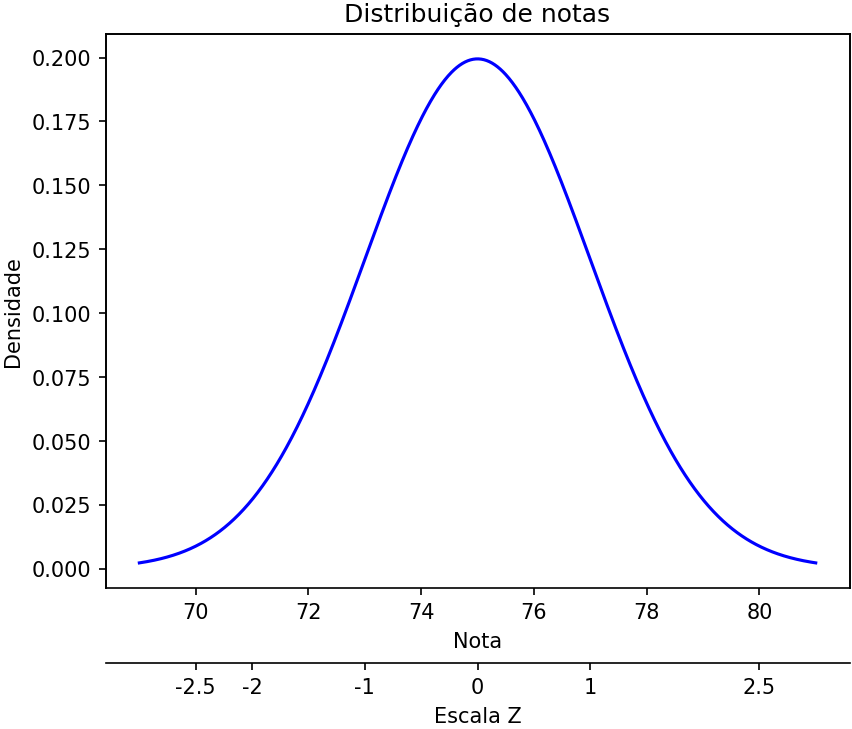
\includegraphics[width=0.6\linewidth]{figs/two_xticks_under} \end{center}

\end{frame}

\begin{frame}
\frametitle{Passo 3: Definir a Região Crítica}
\begin{columns}
\begin{column}{0.5\textwidth}
   A curva normal padrão e os valores de z\\~\\
   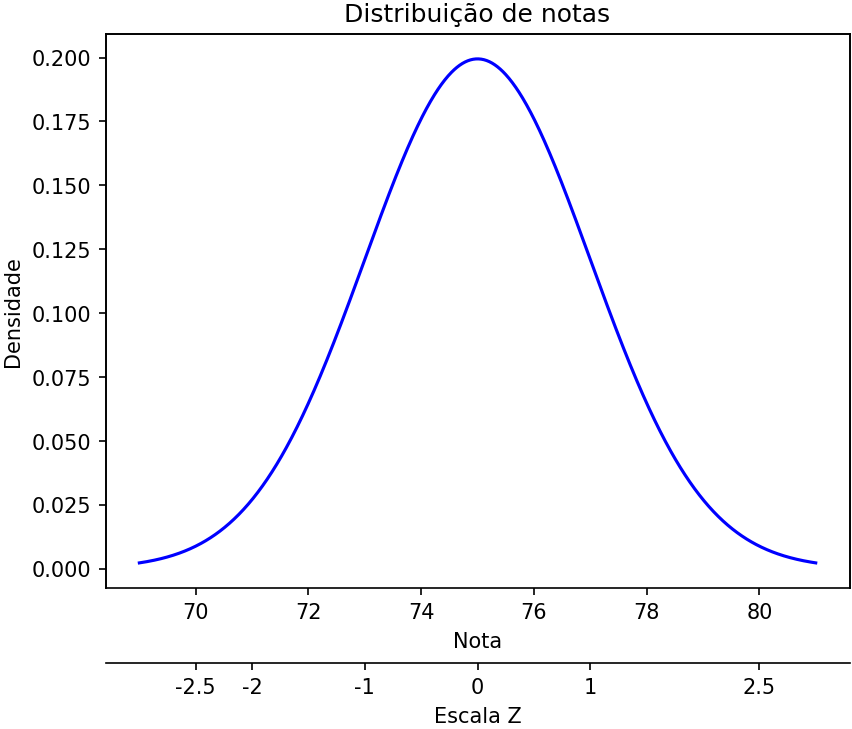
\includegraphics[width=1\linewidth]{figs/two_xticks_under}
\end{column}
\begin{column}{0.5\textwidth}  %%<--- here
   \begin{itemize}
   \item Se a hipótese nula for verdadeira, você esperaria um valor de z próximo a 0;
   \item Se a hipótese nula não for verdadeira, você esperaria um valor de z distante de 0.
   \end{itemize}
\end{column}
\end{columns}
\end{frame}

\begin{frame}
\frametitle{Passo 3: Definir a Região Crítica}
\begin{columns}
\begin{column}{0.5\textwidth}
   Excerto da tabela normal padrão e os valores de z\\~\\

\begin{center}
\begin{tabular}{ccc} 
 \hline
z &	Corpo & Cauda\\
1.630000 & 	0.948400 & 0.051600\\
1.640000 & 0.949500 & 0.050500\\
\boxit{2.1in} 1.650000 & 0.950500 & 0.049500\\
1.660000 & 0.951500 & 0.048500\\
1.670000 & 0.952500 & 0.047500\\
1.680000 & 0.953500 & 0.046500\\
1.690000 & 0.954500 & 0.045500\\
 \hline
\end{tabular}
\end{center}   
   
   
\end{column}
\begin{column}{0.5\textwidth}  %%<--- here
   \begin{itemize}
   \item O valor de corte de 0.05 usado para identificar quais valores z são improváveis se o valor nulo for verdadeiro é chamado de nível alfa (\(\alpha\)).
   \end{itemize}
\end{column}
\end{columns}
\end{frame}

\setbeamercovered{transparent}
\begin{frame}
\frametitle{Passo 3: Definir a Região Crítica}
O valor crítico é o ponto de corte do valor de z; valores de z iguais ou maiores que o valor crítico são considerados improváveis de ocorrer se a hipótese nula for verdadeira.
\begin{center}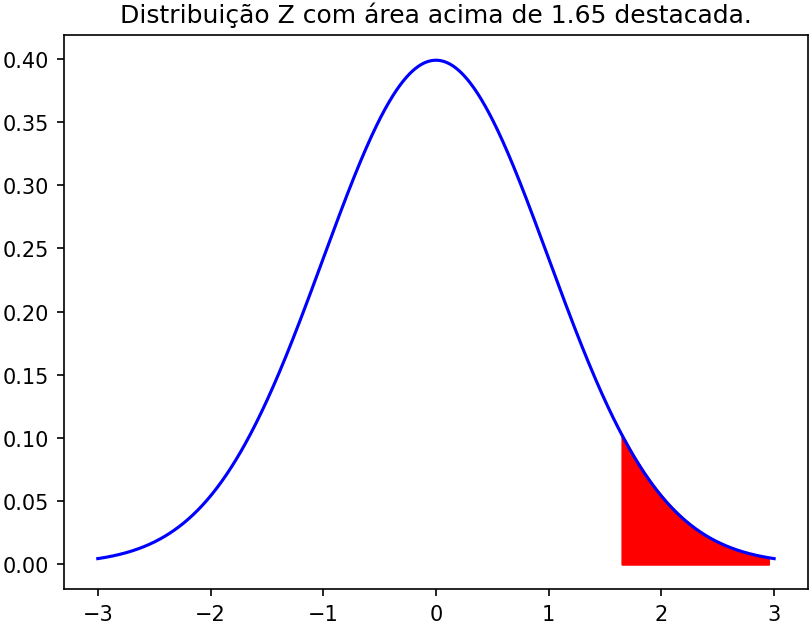
\includegraphics[width=0.6\linewidth]{figs/regiao_critica} \end{center}

\end{frame}

\setbeamercovered{transparent}
\begin{frame}
\frametitle{Etapa 4: calcular a estatística de teste (z para uma média amostral)}
\begin{itemize}
\item 4a. Calcule o desvio observado entre a média amostral e a média da população
\[\bar{x} - \mu = 80 - 75 = 5\]
\item 4b. Calcule o desvio esperado devido ao erro de amostragem
\[SEM_p = \frac{\sigma}{\sqrt{N}} = \frac{10}{\sqrt{25}} = 2\]
\item 4c. Calcule o z para uma média amostral
\[z = \frac{(\bar{x} - \mu)}{SEM_p} = 2.5\]
\end{itemize}
\end{frame}

\setbeamercovered{transparent}
\begin{frame}
\frametitle{Etapa 4: calcular a estatística de teste (z para uma média amostral)}
O valor z obtido de 2.5 é mais extremo que o valor crítico de 1.65, portanto esse valor de z está localizado na região de rejeição (ou seja, a região crítica).
\begin{center}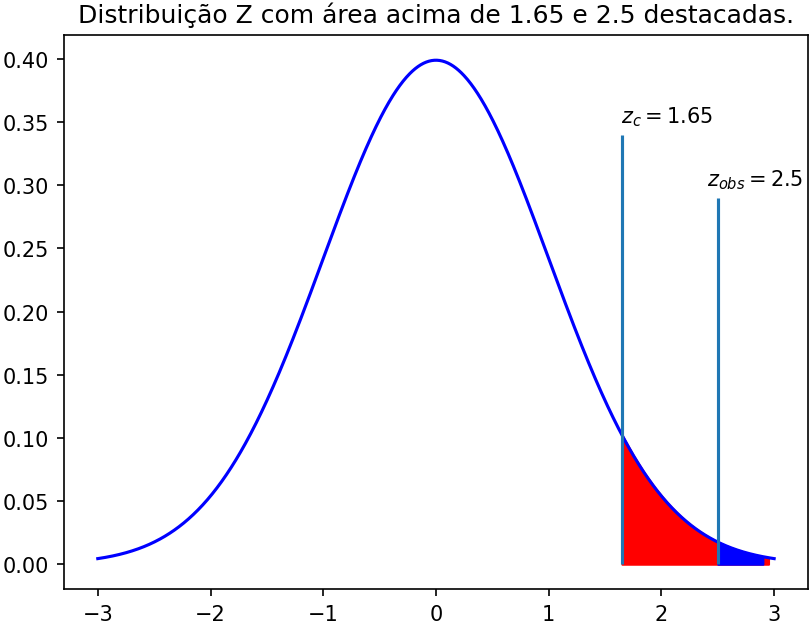
\includegraphics[width=0.55\linewidth]{figs/regiao_critica_observada} \end{center}

\end{frame}


\setbeamercovered{transparent}
\begin{frame}
\frametitle{Etapa 5: calcule o tamanho do efeito e descreva se o seu grau}
Um tamanho de efeito é um índice da diferença entre a média da amostra e a média da população. A estatística de tamanho do efeito normalmente usada ao comparar duas médias é d. 
\[d = \frac{Desvio\quad observado\quad entre\quad as\quad medias}{Desvio\quad padrao} = \frac{\bar{x}-\mu}{\sigma} = \frac{80-75}{10} = 0.5\]

\end{frame}

\setbeamercovered{transparent}
\begin{frame}
\frametitle{Etapa 5: calcule o tamanho do efeito e descreva se o seu grau}
A melhor maneira de interpretar qualquer tamanho de efeito é compará-lo com os tamanhos de efeito produzidos por estudos semelhantes na literatura de pesquisa. Se você não conseguir encontrar estudos semelhantes na literatura para fornecer uma referência, poderá usar as diretrizes gerais sugeridas por Cohen (1992) para interpretar os tamanhos dos efeitos na Tabela 6.2.

\begin{center}
\begin{tabular}{cc} 
 \hline
d  & Tamanho estimado do efeito\\
 \hline
Perto de 0.2 & Pequeno \\
Perto de 0.5 & Médio \\
Perto de 0.8 & Grande \\
 \hline
\end{tabular}
\end{center}   

\end{frame}

\setbeamercovered{transparent}
\begin{frame}
\frametitle{Etapa 6: Interpretando os Resultados do Teste de hipótese usando a z para uma média amostral}

Declaração resumida sobre o teste estatístico acima:\\~\\
As notas dos exames dos alunos que realizaram testes frequentes sobre o material $(\bar{x} = 80, dp = 9.50)$ foram significativamente maiores do que as pontuações daqueles que não realizaram testes frequentes $(\mu = 75, \sigma = 10)$, z (N = 25) = 2.50, p = 0.0062, d = 0.50.\\~\\

Geralmente, você deve fornecer o valor exato de p, se souber. Em alguns casos, você não saberá disso e então escreveria \("p < 0.05"\) se rejeitou a hipótese nula ou \("p > 0.05"\) se não rejeitou a hipótese nula.
\end{frame}

\setbeamercovered{transparent}
\begin{frame}
\frametitle{Etapa 6: Interpretando os Resultados do Teste de hipótese usando a z para uma média amostral}

\begin{center}
\begin{tabular}{cccc} 
 \hline
& Estado da hipótese nula &  & \\
 \hline
& & \textbf{$H_0$ falsa} & \textbf{$H_0$ verdadeira}\\
Decisão & Rejeitar o nulo & Decisão correta/ & Erro tipo I \\
estatística &  & poder estatístico &  \\
& Não rejeitar o nulo & Erro tipo II & Decisão correta\\
 \hline
\end{tabular}
\end{center}

\end{frame}

\setbeamercovered{transparent}
\begin{frame}
\frametitle{Etapa 6: Interpretando os Resultados do Teste de hipótese usando a z para uma média amostral}

\begin{center}
%\setlength{\tabcolsep}{1pt}
\tiny
\begin{tabular}{cccc} 
 \hline
Termo estatístico & Focando na & Focando na & Focando na\\
 & Hipótese Nula & Hipótese Alternativa (de trabalho) & Hipótese Nula (2)\\
 \hline
Erro Tipo I & Rejeitar a hipótese nula & Dizer que o tratamento & Rejeitar um\\
 & quando não deveria ter rejeitado & funciona quando não funciona & Verdadeiro nulo\\
Erro Tipo II & Falhar em rejeitar a hipótese & Dizer que o tratamento & Não rejeitar\\
 & nula quando deveria ser rejeitada & não funciona quando funciona & um Falso nulo\\
Poder Estatístico & Rejeirar o nulo quando & Dizer que o tratamento & Rejeitar um\\
 & deveria ser rejeitado & funciona quando funciona & verdadeiro falso\\ 
 \hline
\end{tabular}
\end{center}

\end{frame}

\setbeamercovered{transparent}
\begin{frame}
\frametitle{Regras de Teste de Hipótese}
O processo de teste de hipótese nada mais é do que um conjunto formal de regras que os pesquisadores usam para determinar se a hipótese nula (\(H_0\)) é provável ou improvável de ser verdadeira.

\begin{itemize}
\item Se a hipótese nula for verdadeira \(\Rightarrow\) valores de z próximos de 0 têm uma probabilidade alta; 
\item Se a probabilidade de um valor de z for baixa o suficiente, os pesquisadores devem rejeitam a hipótese nula.
\end{itemize}

\end{frame}

\setbeamercovered{transparent}
\begin{frame}
\frametitle{O que é um valor p?}
Um valor p é a probabilidade de observar o valor calculada para a estatística do teste ou um valor mais extremo assumindo que a hipótese nula é verdadeira. É usado por pesquisadores para determinar se devem ou não rejeitar uma hipótese nula.\\~\\
Sempre que você for confrontado com a questão de determinar se deve ou não rejeitar a hipótese nula, poderá usar uma das duas regras a seguir:

\begin{enumerate}
\item Se o valor obtido for mais extremo que o valor crítico, você deve rejeitar a hipótese nula;
\item Se o valor p for menor que o valor alfa, você deve rejeitar a hipótese nula.
\end{enumerate}

\end{frame}

\begin{frame}
\frametitle{O que é um valor p?}
Um valor p é a probabilidade de observar o valor calculada para a estatística do teste ou um valor mais extremo assumindo que a hipótese nula é verdadeira.

\begin{center}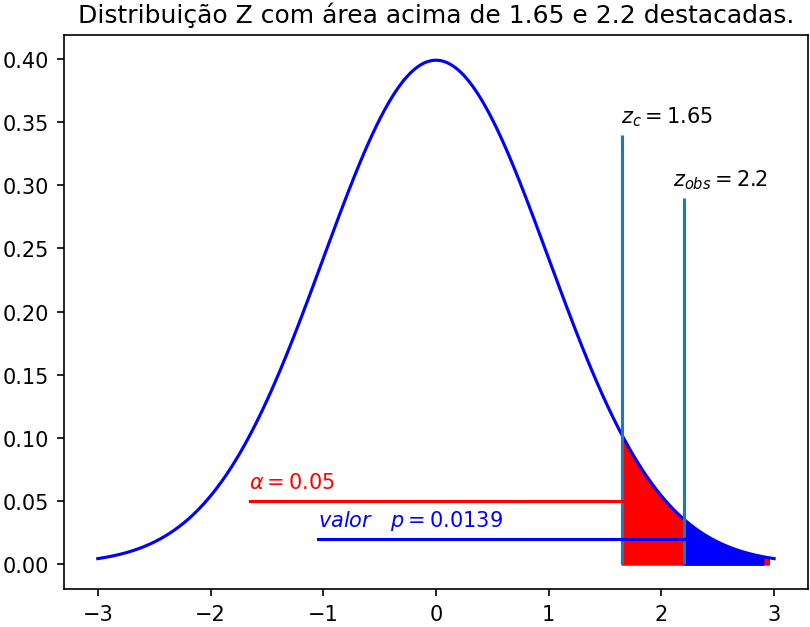
\includegraphics[width=0.6\linewidth]{figs/regiao_critica_valorp.png} \end{center}
\end{frame}

\setbeamercovered{transparent}
\begin{frame}
\frametitle{Por que os estatísticos "falharam em rejeitar o nulo" em vez de "aceitar o nulo"}
Um falso nulo pode não ser rejeitado por um grande número de razões, incluindo erro de amostragem, se o programa precisasse de mais tempo para ser eficaz ou se houvesse uma série de problemas metodológicos com o estudo.\\~\\ 

A frase 'não rejeitar o nulo' significa que atualmente não existem provas suficientes para rejeitar a hipótese nula, mas reconhece que pesquisas futuras poderão fornecer essa evidência. Em contraste, a frase 'Aceitar o nulo' pode implicar uma conclusão final e definitiva que desmente a maioria das situações de investigação.\\~\\

Ignorar possibilidades alternativas não é consistente com a natureza cautelosa das conclusões científicas.

\end{frame}

\setbeamercovered{transparent}
\begin{frame}
\frametitle{Exemplo 7.14}
Suponha que a aceitação de um lote de 1000 peças ocorra apenas, se o comprimento médio de 10 peças, retiradas aleatoriamente do lote, estiver entre 5 e 10 \(cm\). Sabe-se que o comprimento das peças é uma variável aleatória com distribuição Normal de média 7.5 e variância 20 \(cm^2\). Qual é a probabilidade de aceitação de um dado lote?
\vspace{1in}
\vspace{1in}

\end{frame}

\begin{frame}
\frametitle{Distribuição Normal}

\begin{center}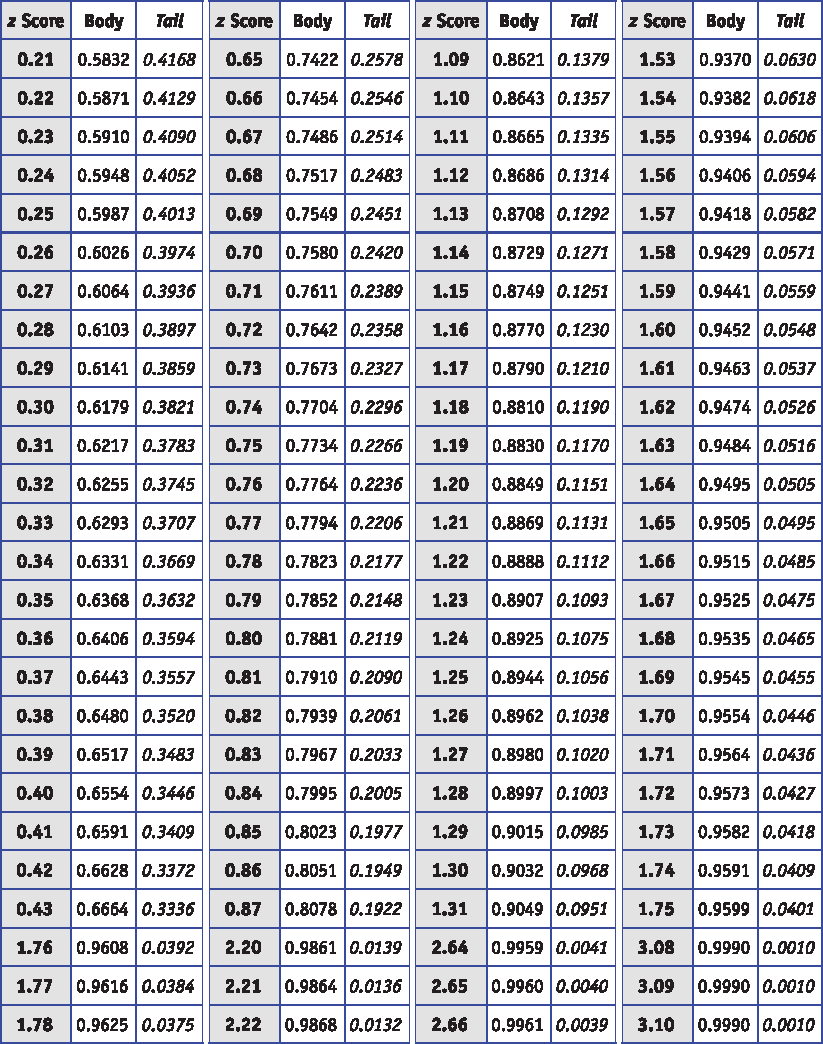
\includegraphics[width=0.5\linewidth]{figs/ztab_crop2} \end{center}
\end{frame}


\setbeamercovered{transparent}
\begin{frame}
\frametitle{Exemplo 7.15}
Uma variável aleatória X assume valores 3, 6 e 8 com, respectivamente, probabilidades 0.4; 0.3 e 0.3. Uma amostra com 40 observações é sorteada. A variável X não tem distribuição Normal e obtemos \(\mu=5.4\) e \(\sigma^2=4.44\). Calcule a probabilidade da média amostral superar o valor 5.
\vspace{1in}
\vspace{1in}

\end{frame}

\setbeamercovered{transparent}
\begin{frame}
\frametitle{Referências bibliográficas}
\printbibliography
\end{frame}

\end{document}